\documentclass[11pt]{article}
\RequirePackage{fullpage}
\RequirePackage[font=small,labelfont=bf]{caption}
\RequirePackage{amsmath,amssymb,amsthm}
\RequirePackage{mathtools}
\RequirePackage{graphicx}
\RequirePackage[normalem]{ulem}
\RequirePackage[hidelinks]{hyperref}
\RequirePackage{wrapfig}
\RequirePackage{subcaption}
\RequirePackage{authblk}
\RequirePackage{bm}
\RequirePackage{bbm}
\RequirePackage{tikz}


% line numbers:
\RequirePackage{lineno}
%\modulolinenumbers[5]
\renewcommand\linenumberfont{\normalfont\tiny\sffamily\color{black}}

% spacing
\RequirePackage{setspace}
%\doublespacing
 
% \RequirePackage[osf]{mathpazo}
\RequirePackage[bibstyle=authoryear,citestyle=authoryear-comp,
                date=year,
                maxbibnames=9,maxnames=5,maxcitenames=2,
                backend=biber,uniquelist=false,uniquename=false,
                % style=apa,
                sorting=nyt,
                hyperref=true]{biblatex}
\RequirePackage[colorinlistoftodos]{todonotes}  %disable
\RequirePackage{color}
\RequirePackage{nicefrac}

\newcommand{\gc}[1]{{\it \color{red} #1 } }
\newcommand{\vb}[1]{{\it \color{blue} #1}}
\newcommand{\vbout}[1]{{\it \color{blue} \sout{#1}}}

% a /nonumber you can turn on/off
\newcommand{\nnn}{\nonumber}
%\newcommand{\nnn}{}


\newcommand{\graham}[1]{\todo[size=\scriptsize, color=red!50]{#1}}
\newcommand{\vince}[1]{\todo[size=\scriptsize, color=blue!50]{#1}}

\renewcommand{\P}{\mathbb{P}}
\newcommand{\E}{\mathbb{E}}
\newcommand{\V}{\text{V}}
\newcommand{\cf}{\emph{cf.} }
\DeclareMathOperator{\var}{Var}
\DeclareMathOperator{\cov}{Cov}
\DeclareMathOperator{\flt}{\mathrm{flat}}
\DeclareMathOperator{\T}{{\mathrm{T}}}
\newcommand{\vect}[1]{\mathbf{#1}}
\newcommand{\nssh}{SSH_n}

\newcommand{\chapquote}[2]{\begin{quotation} \textit{#1} \end{quotation} \begin{flushright} - #2\end{flushright} }

\addbibresource{biblio.bib}


% TODO
% - we have inconsistent notation between intro of results and figure 1 with
%   cov() 
% - address the weird barghi rep correlation point for last time

\title{Estimating the genome-wide contribution of selection to temporal allele frequency change}


\author[$\ast$,$\dag$,$1$]{Vince Buffalo}
\author[$\dag$]{Graham Coop}
\affil[$\ast$]{\footnotesize Population Biology Graduate Group}
\affil[$\dag$]{\footnotesize Center for Population Biology, Department of Evolution and Ecology, University of California, Davis, CA 95616}
\affil[$1$]{\footnotesize Email for correspondence: \href{mailto:vsbuffalo@ucdavis.edu}{vsbuffalo@ucdavis.edu}}

\begin{document}
\maketitle

\linenumbers

\begin{abstract}

 Rapid phenotypic adaptation is often observed in natural populations and
 selection experiments.  However, detecting the impact of this selection
 genome-wide is difficult, since adaptation often proceeds from standing
 variation and selection on highly polygenic traits, both of which may leave
 faint genomic signals indistinguishable from a noisy background of genetic
 drift.  One promising signal comes from the genome-wide covariance between
 allele frequency changes observable from temporal genomic data, e.g.
 evolve-and-resequence studies. These temporal covariances reflect how the
 change in neutral allele frequency at one timepoint is predictive of the
 changes at later timepoints when there is heritable fitness variation in the
 population, as neutral alleles can remain associated with selected alleles
 over time. Since genetic drift does not lead to temporal covariance, we can
 use these covariances to estimate what fraction of the variation in allele
 frequency change through time is driven by linked selection. Here, we
 reanalyze two \emph{Drosophila simulans} evolve-and-resequence studies, and
 one artificial selection experiment in mice, to quantify the effects of linked
 selection over short timescales using covariance among time-points and across
 replicates. We estimate that over 20\% of allele frequency change in these
 experiments is driven by selection in some experiments. Against this
 background of positive genome-wide temporal covariances we also identify
 signals of negative temporal covariance corresponding to reversals in the
 direction of selection for a reasonable proportion of loci over the time
 course of a selection experiment.  Overall, we find that in the three studies
 we analyzed, linked selection has a large impact on short-term allele
 frequency dynamics that is readily distinguishable from genetic drift.

\end{abstract}


\section{Introduction}

A long-standing problem in evolutionary genetics is quantifying the roles of
genetic drift and selection in shaping genome-wide allele frequency changes.
Selection can both directly and indirectly affect allele frequencies, with the
indirect effect coming from the action of selection on correlated loci
elsewhere in genome e.g. linked selection (\cite{Maynard_Smith1974-lc},
\cite{Charlesworth1993-gb,Nordborg1996-nq}; see \cite{Barton2000-zg} for a
review). Previous work on this question has mostly focused on teasing apart
the impacts of drift and selection on genome-wide diversity using population
samples from a single contemporary timepoint, often by modeling the correlation
between regional recombination rate, gene density, and diversity created in the
presence of linked selection \parencite{Begun1992-ey,Elyashiv2016-vt}. This
approach has shown linked selection has a major role in shaping patterns of
genome-wide diversity across the genomes of some of organisms
\parencite{Begun2007-bg,Beissinger2016-cm,Sattath2011-dr,Williamson2014-oy,Andersen2012-bj,Cutter2010-gi},
and has allowed us to quantify the relative influence of positive selection
(hitchhiking) and negative selection (background selection;
\cite{Nordborg2005-dc,McVicker2009-ax,Hernandez2011-gs,Elyashiv2016-vt}.
However, we lack an understanding of how genome-wide linked selection acts over
time.

There are numerous examples of rapid phenotypic adaptation
\parencite{Grant2011-wk,Grant2006-hj,Reznick1997-mh,Franks2007-dr} and rapid
genomic evolution in asexual populations
\parencite{Good2017-om,Bennett1990-bc,Baym2016-kh}.  Yet the polygenic nature
of fitness makes detecting the impact selection on genome-wide variation over
short timescales in sexual populations remarkably difficult. This is because
the effect of selection on a polygenic trait (such as fitness) is distributed
across loci in proportion to their effect sizes. This can lead to subtle allele
frequency shifts on standing variation that are difficult to distinguish from
background levels of genetic drift and sampling variance.  However,
increasingly genomic experimental evolution studies with multiple timepoints,
and in some cases multiple replicate populations, are being used to detect
selected loci \parencite{Turner2011-sx,Turner2012-bm} and differentiate modes
of selection \parencite{Burke2010-tz,Barghi2019-qy,Therkildsen2019-zy}.  In
addition these temporal-genomic studies have begun in wild populations, some
with the goal of finding variants that exhibit frequency changes consistent
with fluctuating selection \parencite{Bergland2014-ij,Machado2018-cs}. In a
previous paper, we proposed that one useful signal for understanding the
genome-wide impact of polygenic linked selection detectable from temporal
genomic studies is the temporal autocovariance in allele frequency changes
\parencite{Buffalo2019-io}.  These covariances are directly estimable from
temporal genomic data and are created when the loci that underly heritable
fitness variation perturb the frequencies of linked neutral alleles; in
contrast, when genetic drift acts alone in a closed population, these
covariances are zero in expectation. Mathematically, temporal covariances are
useful because it is natural to decompose the total variance in allele
frequency change across a set of time intervals into the variances and
covariances in allele frequency change among time intervals.  Furthermore,
biologically, these covariances reflect the extent to which allele frequency
changes in one generation predict changes in another due to a shared fitness
background and shared selection pressures.

Here, we provide the first empirical analyses to quantify the impact of linked
selection acting over short timescales (tens of generations) across two evolve
and re-sequence studies \parencite{Barghi2019-qy,Kelly2019-dc}, and one
artificial selection experiment \parencite{Castro2019-uk}. We repeatedly find a
signal of temporal covariance, consistent with linked selection acting to
significantly perturb genome-wide allele frequency changes across the genome in
a manner that other approaches would not be able differentiate from genetic
drift. We estimate the lower bound on the proportion of total variation in
allele frequency change caused by linked selection, and the correlation between
allele frequency changes between replicate populations caused by response to
convergent selection pressures. Overall, we demonstrate that linked selection
has a powerful role in shaping genome-wide allele frequency changes over very
short timescales.

\clearpage
\section{Results}


% We measure two types of covariances between allele frequency caused by
% selection: temporal autocovariances, and across-replicate covariances. First,
% positive temporal autocovariance in a neutral allele frequency's trajectory
% occurs when the allele becomes associated with a high or low fitness
% chromosomal background, and this association persists through the generations
% due to linkage disequilibrium. As long as the direction of selection remains
% constant, the fitness background is predictive of the direction in the neutral
% allele's frequency changes, creating positive covariance. Even though these
% magnitude of frequency changes at each site may be subtle, as they would be
% under polygenic selection, cumulatively these perturb neighboring sites in a
% predictable manner and build up temporal autocovariance which acts as a
% genome-wide signal of linked selection. Second, if evolution occurs in
% replicate populations undergoing convergent selection pressure, neutral sites
% linked to fitness backgrounds shared across replicates are expected to change
% in the same direction. This creates across-replicate covariance, which is a
% measure of the extent to which convergent selection pressures across replicate
% populations cause similar allele frequency changes. Finally, it is important to
% note that under the null model where the fitness differences between
% individuals are entirely random and non-heritable (e.g. when selection is not
% acting), both forms of covariances are expected to be zero. 

\begin{center}
  \footnotesize
  \begin{tabular}{l c c c c c c}
    Study & Species & Selection & Replicates & Pop. Size & Gens. & Timepoints \\ 
  \hline
    \textcite{Kelly2019-dc}  & \emph{D. simulans} & lab & 3 & $\sim$1100 & 14 & 2 \\ \hline
    \textcite{Barghi2019-qy} & \emph{D. simulans} & lab & 10 & $\sim$1000 & 60 & 7 \\ \hline
    \textcite{Castro2019-uk} & \emph{M. musculus} & \begin{tabular}{c}tibiae length\\control\end{tabular} & \begin{tabular}{c}2\\1\end{tabular} &\begin{tabular}{c}32\\28\end{tabular}  & 20 & 2 \\
 \hline
\end{tabular}
\end{center}

We first analyzed \textcite{Barghi2019-qy}, an evolve-and-resequence study with
ten replicate populations exposed to a high temperature lab environment and
evolved for 60 generations, and sequenced every ten generations. Using the
seven timepoints and ten replicate populations, we estimated the genome-wide $6
\times 6$ temporal covariance matrix $\mathbf{Q}$ for each of the ten
replicates. Each row of these matrices represent the temporal covariance
$\cov(\Delta_{_{10}} p_s, \Delta_{_{10}} p_t)$, between the allele frequency
change (in ten-generation intervals, denoted $\Delta_{_{10}} p_t$) in some
initial reference generation $s$ (the row of the matrix), and some later
timepoint $t$ (the column of the matrix). We corrected these matrices for
biases created due to sampling noise, and normalize the entries for
heterozygosity (see Supplementary Material Sections
\ref{supp:ind-depth-var-corr} and \ref{supp:matrix-correction} for details on
the bias correction). The covariances are expected to be zero when only drift
is acting in a closed population, as only heritable variation for fitness can
create covariance between allele frequency changes \parencite{Buffalo2019-io}.
Averaging across the ten replicate temporal covariances matrices, we find
temporal covariances that are statistically significant (95\% block bootstraps
CIs do not contain zero), consistent with linked selection perturbing
genome-wide allele frequency changes over very short time periods. The
covariances between all adjacent time intervals are positive and then decay
towards zero as we look at more distant time intervals, as expected when
directional selection affects linked variants' frequency trajectories until
ultimately linkage disequilibrium and the additive genetic variance for fitness
associated with neutral alleles decays \parencite{Buffalo2019-io}. The temporal
covariances per replicate are noisier but this general pattern holds; see
Supplementary Figures \ref{suppfig:barghi-cov-panels}.
\textcite{Barghi2019-qy}'s design means that the covariances we see in adjacent
time intervals are on average ten generations apart, and given the temporal
decay in covariance we see, the covariances on shorter time-scales (e.g. if
adjacent generations had been sequenced) may well be higher yet (see
Supplementary Material Section \ref{supp:barghi-covs} for more details).

%We visualize these covariances in Figure \label{figure-1} (A), which
%depicts the temporal covariances through time, for each of the five
%off-diagonal rows temporal covariance matrix. Each row represents the temporal
%covariance $\cov(\Delta_{_{10}} p_s, \Delta_{_{10}} p_t)$, between some initial
%reference generation $s$ (the row of the matrix), and some later timepoint $t$
%(the column of the matrix). For each row, the covariances at first are
%positive, and then decay towards zero as expected when directional selection
%affects linked variants' frequency trajectories until ultimately linkage
%disequilibrium and additive genetic variance for decay
%\parencite{Buffalo2019-io}. Note that per replicate, the signal is a bit
%noisier; see Supplementary Figures XXX.

 
%Since the \textcite{Barghi2019-qy} study sequenced each
% replicate population every ten generations, we calculate the temporal
% covariance matrix over ten-generation allele frequency changes, which we write
% as $\cov(\Delta_{_{10}} p_s, \Delta_{_{10}} p_t)$. The diagonal elements of
% this temporal covariance matrix are the sum of all variances in allele
% frequency changes and pairwise covariances, e.g. element $\mathbf{Q}_{t,t} =
% \sum_{i=t}^{9} \var(\Delta p_i) + 2\sum_{i \ne j} \cov(\Delta p_i, \Delta
% p_j)$. Each off-diagonal element $\mathbf{Q}_{t,s}, \; t \ne s$ contains the
% sum of pairwise covariances, $\mathbf{Q}_{t,s} = \sum_{i=t}^{t+9}
% \sum_{j=s}^{s+9} \cov(\Delta p_i, \Delta p_j)$ (see Supplementary Material
% Section \ref{supp:barghi-covs} for more details). These off-diagonal
% covariances are expected to be zero when only drift is acting in the
% population, as only linked selection can create covariance between allele
% frequency changes \parencite{Buffalo2019-io}. Furthermore, since we cannot
% directly observe the temporal covariances between adjacent timepoints, but only
% the sums of temporal covariances, we expect the off-diagonal elements of
% $\mathbf{Q}$ to be weak. This is because the magnitude of a temporal covariance
% $\cov(\Delta p_i, \Delta p_j)$ is governed by the level of additive genetic
% variance and linkage disequilibrium that persists after $|i-j|$ generations of
% decay, which in \textcite{Barghi2019-qy}'s study design is on average 10
% generations.

\begin{figure}[!htb]
  \centering
  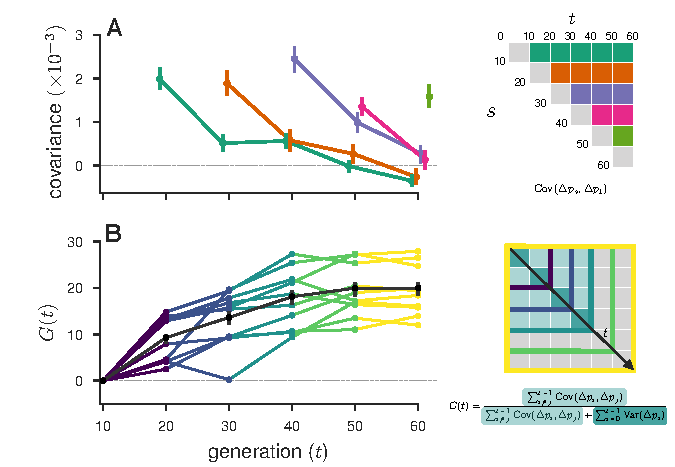
\includegraphics[width=\textwidth]{figures/figure-1.pdf}

  \caption{A: Temporal covariance, averaged across all ten replicate
    populations, through time from the \textcite{Barghi2019-qy} study. Each
    line depicts the temporal covariance $\cov(\Delta p_s, \Delta p_t)$ from
    some reference generation $s$ to a later time $t$ which varies along the
    x-axis; each line corresponds to a row of the upper-triangle of the
    temporal covariance matrix with the same color (upper right). The ranges
    around each point are $95\%$ block-bootstrap confidence intervals. B: The
    proportion of the total variance in allele frequency change explained by
    linked selection, $G(t)$, as it varies through time $t$ along the x-axis.
    The black line is the $G(t)$ averaged across replicates, with the $95\%$
    block-bootstrap confidence interval. The other lines are the $G(t)$ for
    each individual replicate, with colors indicating what subset of the
    temporal-covariance matrix to the right is being included in the
  calculation of $G(t)$.}

  \label{fig:figure-1}
\end{figure}

While the presence of positive temporal covariances is consistent with linked
selection affecting allele frequencies over time, this measure not easily
interpretable. Additionally, we can quantify the impact of linked selection on
allele frequency change as the ratio of total covariance in allele frequency
change to the total variance in allele frequency change. We denote the
change in allele frequency as $\Delta p_t = p_{t+1}-p_t$, where $p_t$ is the
allele frequency in generation $t$. Since the total variation in allele
frequency change can be partitioned into variance and covariance components,
$\var(p_t - p_0) = \sum_{i} \var(\Delta p_i) + \sum_{i \ne j} \cov(\Delta
p_i, \Delta p_j)$, and the covariances are zero when drift acts alone, this is
a lower bound on how much of the variance in allele frequency change is caused
by linked selection \parencite{Buffalo2019-io}. We call this measure $G(t)$, defined as

\begin{align}
  G(t) = \frac{\sum_{i\ne j}^t \cov(\Delta p_i, \Delta p_j)}{\var(p_t - p_0)}
\end{align}
%
which estimates the effect of linked selection between the initial
generation $0$ and some later generation $t$, which can be varied to see how
this quantity grows through time. As with the temporal covariances, the study
design of \textcite{Barghi2019-qy} leads our measure $G(t)$ to be even more
conservative, since the temporal covariances within each ten-generation block
between sequenced timepoints are not directly observable, and are not included
in the numerator of $G(t)$. Still, we find a remarkably strong signal.
Greater than $20\%$ of total variation in allele frequency change over 60
generations is the result of linked selection.

Additionally, we looked for a signal of temporal autocovariance in
\textcite{Bergland2014-ij}, a study that collected \emph{Drosophila
melanogaster} through Spring-Fall season pairs across three years. If there was
a strong  pattern of genome-wide fluctuating selection, we might expect a
pattern of positive covariances between similar seasonal changes, e.g.
Spring-Fall in two adjacent years, and negative covariances between dissimilar
seasonal changes, e.g. Spring-Fall and Fall-Spring in two adjacent years.
However, we find no such signal over years; we discuss this in more depth in
Supplementary Materials Section \ref{supp:bergland-reanalysis}.

The replicate design of \textcite{Barghi2019-qy} allows us to quantify another
covariance: the covariance in allele frequency change between replicate
populations experiencing convergent selection pressures. These
between-replicate covariances are created in the same way as temporal
covariances: neutral alleles linked to a particular fitness background
experience are expected to have allele frequency changes in the same direction
if the selection pressures are similar. Intuitively, where temporal covariances
reflect that neutral alleles associated with heritable fitness backgrounds are
predictive of frequency changes between generations, replicate covariances
reflect that heritable fitness backgrounds common to each replicate predict
(under the same selection pressures) frequency changes between replicates. We
measure this through a statistic similar to a correlation, which we call the
convergent correlation: the ratio of average between-replicate covariance
across all pairs to the average standard deviation across all pairs of
replicates, 

\begin{align}
  \label{eq:conv-corr}
  \mathrm{cor}(\Delta p_s, \Delta p_t) = \frac{\E_{A\ne B} \left( \cov(\Delta p_{s,A}, \Delta p_{t,B}) \right)}{\E_{A\ne B} \left( \sqrt{\var(\Delta p_{s,A}) \var(\Delta p_{t,B})} \right)}
\end{align}
%
where $A$ and $B$ here are two replicate labels, and for the
\textcite{Barghi2019-qy} data, we use $\Delta_{_{10}} p_t$.

We've calculated the convergent correlation for all rows of the replicate
covariance matrices. Like temporal covariances, we visualize these through time
(Figure \ref{fig:figure-2} A), with each line representing the convergent
correlation from a particular reference generation $s$ as it varies with $t$
(shown on the x-axis). In other words, each of the colored lines corresponds to
the like-colored row of the convergence correlation matrix (upper left in
Figure \ref{fig:figure-2} A). We find these convergent covariances are
relatively weak, and decay very quickly from an initial value of about 0.1
(95\% block bootstrap confidence intervals $[0.094, 0.11]$) to around 0.01
(95\% CIs [0.0087, 0.015]) within 20 generations. This seems to confirm a
primary finding of the original \textcite{Barghi2019-qy} study: that
alternative loci contribute to adaptation in different replicates.

\begin{figure}[!htb]
  \centering
  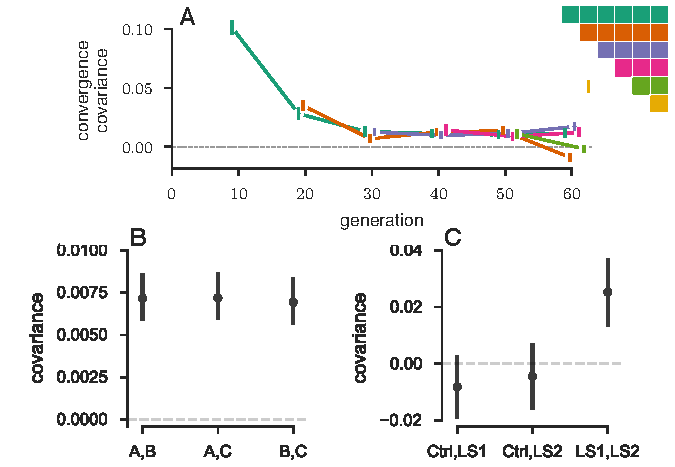
\includegraphics[width=\textwidth]{figures/figure-2.pdf}

  \caption{{\bf A}: The convergence correlation, averaged across replicate
    pairs, through time. Each line represents the convergence correlation
    $\mathrm{cor}(\Delta p_{s}, \Delta p_{s})$ from a starting reference
    generation $s$ to a later time $t$, which varies along the x-axis; each
    line corresponds to a row of the temporal convergence correlation matrix
    depicted to the right.  {\bf B}: The convergence covariance between
    individual pairs of replicates in the \textcite{Kelly2019-dc} data. {\bf
    C}:  The convergence covariance between individual pairs of replicates in
    \parencite{Castro2019-uk} data, for the two selection lines  (LS1 and LS2)
    and the control (Ctrl); gray CIs are those using the complete dataset, blue
    CIs exclude chromosomes 5 and 10 which harbor the two regions
    \textcite{Castro2019-uk} found to have signals of parallel selection between
    LS1 and LS2.}

  \label{fig:figure-2}
\end{figure}

% TODO \vince{GC: you had ??? here, not sure I see the issue.} 

A benefit of between-replicate covariances is that unlike temporal covariances,
these can be calculated with only two sequenced timepoints and a replicated
study design. This allowed us to assess the impact of linked selection in
driving convergent patterns of allele frequency change across replicate
populations in two other studies. First, we reanalyzed the selection experiment
of \textcite{Kelly2019-dc}, which evolved three replicate wild populations of
\emph{Drosophila simulans} for 14 generations adapting to a novel laboratory
environment. Since each replicate was exposed to the same selection pressure
and share linkage disequilibria common to the original natural founding
population, we expected each of the three replicate populations to have
positive between-replicate covariances. We find all three pairwise
between-replicate covariances are positive and statistically significant (95\%
CIs, [0.0063, 0.0086], [0.0064, 0.0086], [0.0061, 0.0083]). We estimate the
convergent correlation coefficient across these replicates as 0.36 ($95\%$
block-bootstrap confidence interval $[0.31, 0.40]$).

%\gc{TODO GIVE conversion \% var due to linked selection. }
Second, we reanalyzed the Longshanks selection experiment, which selected for
longer tibiae length relative to body size in mice, leading to a response to
selection of about 5 standard deviations over the course of twenty generations
\parencite{Castro2019-uk}. This study includes two independent selection lines,
Longshanks 1 and 2 (LS1 and LS2), and an unselected control line (Ctrl).
Consequently, this selection experiment offers a useful control to test our
between-replicate covariances: we expect to see positive between-replicate
covariance in the comparison between the two Longshanks selection lines, but
not between the two pairwise comparisons between the control line and the two
Longshanks lines. We find that this is the case (gray confidence intervals in
Figure \ref{fig:figure-2} C), with the two Longshanks comparisons to the
control line not being significantly different from zero, while the comparison
between the two Longshanks line is statistically significantly different from
zero (CIs [0.013, 0.037]).

A major finding in the Longshanks study were two major-effect loci that showed
parallel frequency shifts between the two selection lines: a region harboring
the gene Nkx3-2 known to be involved in limb development, and another region
harboring six other candidate genes. We were curious to what extent our
genome-wide covariances were being driven by these two outlier large-effect
loci, so we excluded them from the analysis. Since we do not know the extent to
which linkage disequilibrium around these large-effect loci affects neighboring
loci, we took the conservative precaution of excluding the entire chromosomes
these loci reside on (chromosomes 5 and 10), and re-calculating the temporal
covariances. We find excluding these large effect loci has little impact on the
confidence intervals (blue confidence intervals in Figure \ref{fig:figure-2}),
indicating that these across-replicate covariances are indeed driven by a
polygenic signal.

%We find that for covariances 2 timepoints apart ($k=2
%\times 10$ generations), the $20\%$ right tail is inflated by a of 1.3 (95\% CI
%[1.29, 1.32]), consistent with linked selection creating positive covariance in
%allele frequency change. Under constant directional selection, we expect these
%positive covariances between increasingly distant timepoints to decay to zero
%as additive genetic variance is exhausted by selection and linkage
%disequilibrium decays. Instead we find that for covariances 4 timepoints apart
%($k=4 \times 10$ generations), the left tail of negative covariances is
%inflated by a factor of 1.19 (95\% CI [1.17, 1.21]).

\begin{figure}
  \centering
  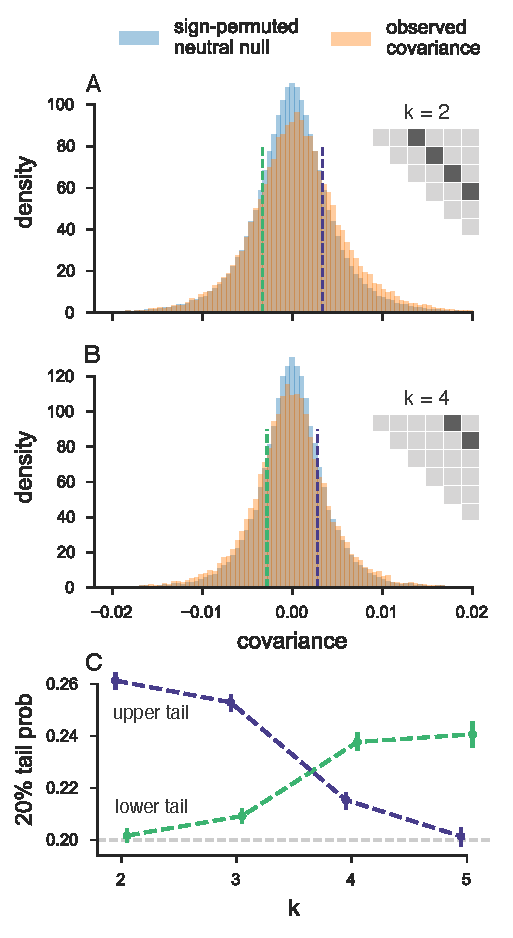
\includegraphics[]{figures/figure-3.pdf}

  \caption{\footnotesize {\bf A}, {\bf B}: The distribution of temporal covariances
    calculated in 100kb genomic windows from the \textcite{Barghi2019-qy}
    study, plotted alongside an empirical neutral null distribution created by
    recalculating the windowed covariances on a 1,000 sign permutations of
    allele frequency changes within tiles. The histogram bin number is 88,
    chosen by cross validation (Supplementary Materials
    \ref{suppfig:barghi-cross-validation-binsize}). In subfigure {\bf A}, windowed
    covariances $\cov(\Delta p_t, \Delta p_{t+k})$ are separated by $k=2 \times
    10$ generations and in subfigure {\bf A} the covariances are separated by $k=4
    \times 10$ generations; each $k$ is an off-diagonal from the variance
    diagonal of the temporal covariance matrix (see cartoon of upper-triangle
    of covariance matrix in subfigures {\bf A} and {\bf B}, where the first diagonal is the
    variance, and the dark gray indicates which off-diagonal of the covariance
    matrix is plotted in the histograms). {\bf C}: The lower and upper tail
    probabilities of the observed windowed covariances, at 20\% and 80\%
    quintiles of the empirical neutral null distribution, for varying time
    between allele frequency changes (i.e. which off-diagonal $k$). The
  confidence intervals are  $95\%$ block-bootstrap confidence intervals, and the
light gray dashed line indicates the 20\% tail probability expected under the
neutral null.}
    \label{fig:figure-3} 
\end{figure}

\clearpage


Finally, we observed that in the longest study  we analyzed
\parencite{Barghi2019-qy}, some genome-wide temporal covariances become
negative at future timepoints (see the first two rows in Figure
\ref{fig:figure-1} A). This shows that alleles that were on average going up
initially are later going down in frequency, i.e. that the average direction of
selection experienced by alleles has flipped. This must reflect either a change
in the environment or the genetic background, due to epistatic relationships
among alleles altered by frequency changes or recombination breaking up
selective alleles.  Such reversals of selective dynamics could be occurring at
other timepoints but the signal of a change in the direction of selection at
particular loci may be washed out when we calculate our genome-wide average
temporal covariances. To address this limitation, we calculated the
distribution of the temporal covariances over 100kb genomic windows \vb{which
we refer to as \emph{windowed covariances}} (Figure \ref{fig:figure-3}
\vb{shows these distributions} pooling across all replicates; see Supplementary
Figure \ref{suppfig:barghi-offset-replicate-panels} for individuals
replicates). The covariance of each tile will be noisy, due to sampling and
genetic drift, and the neutral distribution of the covariance is complicated
due to linkage disequilibria (which can occur over long physical distances in
E\&R and selection studies, \cite{Nuzhdin2013-gf,Baldwin-Brown2014-cl}). To
address this, we have developed a permutation-based procedure that constructs a
null distribution by randomly flipping the signs of the  allele frequency
changes per-genomic window. This destroys the systematic covariances created by
linked selection and creates a sampling distribution of the covariances
spuriously created by neutral genetic drift while preserving the complex
dependencies between adjacent loci created by linkage disequilibrium (see
Supplementary Material Section \ref{supp:empirical-null} for more details on
this approach).  This empirical neutral null distribution is conservative in
the sense that the variances of the covariances are wider than expected under
drift alone as they include the effect of selection on the allele frequency
change within a time-interval, just not between time-intervals. We see (Figure
\ref{fig:figure-3} A and B) that windowed temporal covariances between close
timepoints are skewed positive (a heavy right tail), while between more distant
timepoints these windowed temporal covariances tend to shift to become more
negative (a heavy left tail).  We quantified the degree to which the left and
right tails are inflated compared to the null distribution as a function of
time, and see excesses in both tails in Figure \ref{fig:figure-3} C. This
finding is also robust to sign-permuting allele frequency changes on a
chromosome-level, the longest extent that gametic linkage disequilibria can
extend (Supplementary Figure \ref{suppfig:barghi-tailprobs-seqid}). We see a
striking pattern that the windowed covariances not only decay towards zero, but
in fact become negative through time, consistent with many regions in the
genome having had a reversed fitness effect at later timepoints.


\section{Discussion}

Since the seminal analysis of \textcite{Maynard_Smith1974-lc} demonstrating
that diversity is reduced at linked neutral variation as an advantageous
polymorphism sweeps to fixation, over four decades of theoretical and empirical
research has enriched our understanding of linked selection. This work has led
to the discovery of selected genes from genomic signals of hitchhiking
\parencite{Nair2003-tw,Voight2006-rn}, found genome-wide signals of linked
selection
\parencite{Aguade1989-jx,Begun1992-ey,Cutter2010-gi,Andersen2012-bj,Cutter2003-tl}
leading to the development of recurrent hitchhiking \parencite{Stephan1992-jc}
and background selection \parencite{Charlesworth1993-gb} models that attempt
explain this pattern. Since, much attention has focused on quantifying the
impact of background selection \parencite{McVicker2009-ax} and developing
theoretic machinery \parencite{Coop2012-cd} to differentiate the regional
reductions in diversity into those caused by full and partial sweeps, and those
caused by background selection \parencite{Elyashiv2016-vt}. However, as other
models of soft sweeps from standing variation emerged
\parencite{Hermisson2005-hs,Pennings2006-lj}, attention shifted towards
detecting other modes of linked selection \parencite{Pritchard2010-tk}, a more
difficult endeavor \parencite{Przeworski2005-bg} addressed using new coalescent
models \parencite{Berg2015-xj} and machine learning methods
\parencite{Schrider2017-yx}. An alternative approach to understanding the
genome-wide effects of selection on standing variation, e.g. selection on an
infinitesimal polygenic trait, stems from an early quantitative genetic model
of linked selection \parencite{Robertson1961-ho} and its later developments
(\cite{Santiago1995-hx,Santiago1998-bs}; see also \cite{Barton2000-zg} for a
comparison of these models with classic hitchhiking models). Implicit in these
models is that autocovariance between allele frequency change is created when
there is heritable fitness variation in the population, a signal that can be
readily detected from temporal genomic data \parencite{Buffalo2019-io}. Here,
we provide the first empirical evidence of linked selection acting on standing
variation over very short timescales.

We reanalyzed three published temporal genomic datasets and detected the
genome-wide signature of linked selection acting over tens of generations.
Furthermore, we find the dynamics of temporal autocovariance are consistent
with theory; the temporal covariance in allele frequencies decays as both
the fitness variation associated with particular haplotypes and the linkage
disequilibria between selected and neutral loci decay through time. In
reanalyzing one study \parencite{Barghi2019-qy}, we find that after sixty
generations, greater than 20\% of the variation in allele frequency change is
directly due to the action linked selection. Capitalizing on replicated
evolve-and-resequence study designs, we characterized the extent to which
convergent selection pressures lead to parallel changes in allele frequencies
across replicate populations, finding moderate correlations in allele frequency
changes.

While we must keep in mind that the studies analyzed here were all laboratory
populations and natural selection in the wild will likely differ, overall we
have found that linked selection has a remarkably strong effect for such short
study durations. Depending on how many loci affect fitness, such a strong
effect of linked selection may not be differentiable from genetic drift using
only single contemporary population samples. In this way, temporal data allows
us to sidestep the key problem of detecting selection from standing variation:
that the genomic footprint leaves too soft of a signature to differentiate from
a background of genetic drift. In fact we find that the temporal covariance
signal is detectable even in the most extremely difficult to detect soft sweep
case: polygenic selection on an infinitesimal trait. In our reanalysis of the
\textcite{Castro2019-uk} data, by showing the covariance signal remains even
after excluding the chromosomes containing two large-effect loci, we showed the
covariance signal we detect is indeed driven by polygenic fitness variation
(and confirm a point in the original study that tibiae length, aside from these
two large effect loci, is a highly polygenic trait).

It is worth building some intuition why temporal covariance allows us to detect
such faint signals of polygenic linked selection from temporal genomic data.
Each variant is subject to both variance in allele frequency due to drift and
two levels of sampling noise (as individuals are sampled from the population
and reads are sampled from amplified DNA), which at any locus swamps the
temporal covariance signal and creates spurious covariances. However, these
spurious covariances do not share a common sign across timepoints whereas the
covariances created by linked selection do; consequently, averaging across the
entire genome, the temporal signal exceeds sampling noise.

One limitation of these analyses is that none of the studies we reanalyzed
estimated linkage disequilibria data for the evolved populations. Our theory of
temporal autocovariance tells us that the temporal autocovariances a neutral
site experiences is determined by the product of the expected linkage
disequilibrium and additive fitness variation that persists through the
generations \parencite{Buffalo2019-io}. This leads to a clear prediction:
regions of higher linkage disequilibrium and lower recombination should have
greater temporal autocovariance than regions with lower LD and higher
recombination. Unfortunately, we lack a high-resolution recombination map for
\emph{D. simulans} and while there are LD data for \emph{D. simulans}
\parencite{Signor2018-wg} we did not find a relationship between temporal
covariance and LD. 

% \graham{TODO Is important point. We'll likely need plots for supp}

We believe this is driven by the idiosyncratic nature of LD in
evolve-and-resequence populations \parencite{Nuzhdin2013-gf,Kelly2019-dc}, and
that we might find such a relationship if LD data from the evolved population
were available. Unfortunately, sequencing multiple timepoints is expensive and
the low-coverage and/or pooled-sequencing approaches common in these studies
prohibit estimating linkage disequilibrium. Future studies complete with LD
data and recombination maps would allow one to disentangle the influence of
closely linked sites from more distant sites in causing temporal
autocovariance, and allow us to better understand whether sites in high
recombination regions are free from the effects of linked selection.
Furthermore, such additional data would allow for localizing the effects of
temporal covariance, which would allow us to estimate not just the genome-wide
fraction of variation in frequency change ($G(t)$), but also the fraction of
the genome impacted by linked selection, allowing us to synthesize the temporal
approach with single-timepoint studies like that of \textcite{Elyashiv2016-vt}.

%Why the variation in convergence correlations?

Thus far, the most comprehensive studies implicating linked selection in
affecting genome-wide diversity have been in \emph{Drosophila}
\parencite{Begun1992-ey,Elyashiv2016-vt,Sattath2011-dr} and
\emph{Caenorhabditis} \parencite{Cutter2003-tl,Cutter2003-tl,Andersen2012-bj},
whereas the evidence for linked selection in plant and yeast species is weak
\parencite{Cutter2013-ba}. Both \emph{Drosophila} and \emph{Caenorhabditis}
have short genetic maps (or in the case of selfing \emph{C.  elegans}, small
effective recombination rates), and large effect population sizes, two factors
predicted to increase the degree to which hitchhiking impacts genome-wide
diversity \parencite{Barton2000-zg}. However, our results here show that even
with small effective population sizes (300, 450, and 45 for the
\textcite{Kelly2019-dc}, and \textcite{Castro2019-uk} studies respectively)
and, in the case of mice, moderately-sized genetic maps (around 14 Morgans;
\cite{Cox2009-hf}), we still see a fairly strong effect of linked selection.
This suggests that while these factors may govern the dynamics of classic
hitchhiking events, they could perhaps play less of a role in polygenic linked
selection. However, with only three cases analyzed, further studies on
different taxa are needed.

Finally, in reanalyzing the \textcite{Barghi2019-qy} study, we find evidence
of complex linked selection dynamics. This is due either to a change in the
environment and its consequences for the fitness of regions in the genome,
recombination breaking up selected alleles, or epistatic interactions between
loci. It is important to note that the original study did not intentionally
alter the environment in any way; this signal is attained without intentionally
seeking it out. Discerning which of these is creating negative temporal
autocovariance is a sizable challenge, requiring sequencing each generation and
LD data.

Overall, we hope this will encourage more temporal genomic studies in both
laboratory and natural populations. Understanding the dynamics of linked
selection over short timescales will help to unite phenotypic studies of rapid
adaptation of polygenic adaptations with a detectable genomic signature, to
address long-standing questions concerning linked selection, evolutionary quantitative
genetics, and the overall impact selection has on genetic variation. 

\section{Acknowledgments} 

We would like to thank the authors of the original studies we've analyzed,
including Neda Barghi, Christian Schl{\"o}tterer, John Kelly, Kimberly Hughes,
Frank Chan, Campbell Rolian, Nick Barton, Alan Bergland, and Dmitri Petrov.  We
would also like to thank Doc Edge for helpful statistical advice, and Matt
Osmond for helpful discussions. 

\printbibliography


\section{Appendix}

\section{Estimator Bias Correction}
\subsection{Correcting variance bias with a single depth sampling process}
\label{supp:depth-var-corr}

Following \textcite{Waples1989-sj}, we have that the variance in allele
frequency change at a locus in the initial generation, which is entirely due to
the binomial sampling process, is $\var(p_0) = \nicefrac{p_0(1-p_0)}{d_0}$
where $d_0$ is the number of binomial draws (e.g. read depth). At a later
timepoint, the variance in allele frequency is a result of both the binomial
sampling process at time $t$ and the evolutionary process. Using the law of
total variation we can partition the variation from each process,

\begin{align}
  \var(\widetilde{p_t}) &= \E(\var(\widetilde{p_t} | p_t)) + \var(\E(\widetilde{p_t}|p_t)) \\
                        &= \underbrace{\frac{p_t(1-p_t)}{d_t}}_\text{generation $t$ sampling noise} + \underbrace{\var(p_t)}_\text{variance due to evolutionary process}.
  %\frac{\var(\widetilde{p_t})}{p_0(1-p_0)} &= \frac{p_t(1-p_t)}{p_0(1-p_0) d_t} + 1 - \left( 1-\frac{1}{2N}\right)^t.
  %\frac{\var(\widetilde{p_t})}{p_0(1-p_0)} &= \frac{p_t(1-p_t)}{p_0(1-p_0) d_t} + \frac{t}{2N} + O\left((2 N)^{-2}\right).
\end{align}

Under a drift-only process, $\var(p_t) = p_0(1-p_0)\left[1- \left(1 -
\frac{1}{2N}\right)^t\right]$. However, with heritable variation in fitness, we
need to consider the covariance in allele frequency changes across generations
\parencite{Buffalo2019-io}. We can write

\begin{align}
  \var(p_t) &= \var\left(p_0 + (p_1 - p_0) + (p_2 - p_1) + \ldots + (p_t - p_{t-1}) \right) \\
         &= \var\left(p_0 + \Delta p_0 + \Delta p_1 + \ldots + \Delta p_{t-1} \right) \\
         &= \var(p_0) + \sum_{i=0}^{t-1} \cov(p_0, \Delta p_i) + \sum_{i=0}^{t-1} \var(\Delta p_i) + \sum_{0 \le i < j}^{t-1} \cov(\Delta p_i, \Delta p_j).
\end{align}
%

Each allele frequency change is equally like to be positive as it is to be
negative; thus by symmetry this second term is zero. Additionally $\var(p_0) = 0$,
as we treat $p_0$ as a fixed initial frequency. We can write, 

\begin{align}
  \var(p_t) &= \sum_{i=0}^{t-1} \var(\Delta p_i) + \sum_{0 \le i < j}^{t-1} \cov(\Delta p_i, \Delta p_j).
\end{align}

The second term, the cumulative impact of variance in allele frequency change
can be partitioned into heritable fitness and drift components
\parencite{Santiago1995-hx,Buffalo2019-io}

\begin{align}
  \var(p_t) &= \sum_{i=0}^{t-1} \var(\Delta_{_D} p_i) + \sum_{i=0}^{t-1} \var(\Delta_{_H} p_i) + \sum_{0 \le i < j}^{t-1} \cov(\Delta p_i, \Delta p_j).
\end{align}

where $\Delta_{_H} p_t$ and $\Delta_{_D} p_t$ indicate the allele frequency
change due to heritable fitness variation and drift respectively. Then, sum of
drift variances in allele frequency change is

\begin{align}
  \sum_{i=0}^{t-1} \var(\Delta_{_D} p_i) = \sum_{i=0}^{t-1} \frac{p_i(1-p_i)}{2N}
\end{align}
%
replacing the heterozygosity in generation $i$ with its expectation, we have

\begin{align}
  \sum_{i=0}^{t-1} \var(\Delta_{_D} p_i) &= p_0(1-p_0) \sum_{i=0}^{t-1} \frac{1}{2N} \left(1-\frac{1}{2N}\right)^i \\
                                         &= p_0(1-p_0) \left[1 - \left(1-\frac{1}{2N}\right)^t \right]
\end{align}
%
which is the usual variance in allele frequency change due to drift.  Then, the
total allele frequency change from generations $0$ to $t$ is
$\var(\widetilde{p}_t - \widetilde{p}_0) = \var(\widetilde{p}_t) +
\var(\widetilde{p}_0) - 2 \cov(\widetilde{p}_t, \widetilde{p}_0)$, where the
covariance depends on the nature of the sampling plan (see \cite{Nei1981-oy,
Waples1989-sj}). In the case where there is heritable variation for fitness,
and using the fact that $\cov(\widetilde{p}_t, \widetilde{p}_0) =
\nicefrac{p_0(1-p_0)}{2N}$ for Plan I sampling procedures
\parencite{Waples1989-sj}, we write,

\begin{align}
  \var(\widetilde{p}_t - \widetilde{p}_0) &= \var(\widetilde{p}_t) + \var(\widetilde{p}_0) - 2 C \cov(\widetilde{p}_t, \widetilde{p}_0) \\
                                          &= \frac{p_t(1-p_t)}{d_t}  + \frac{p_0(1-p_0)}{d_0} + p_0(1-p_0) \left[1 - \left(1-\frac{1}{2N}\right)^t \right] + \\ & \;\;\;\;\;\;
                                               \sum_{i=0}^{t-1} \var(\Delta_{_H} p_i)  + \sum_{0 \le i < j}^{t-1} \cov(\Delta p_i, \Delta p_j) - \frac{C p_0(1-p_0)}{2N} \\
  \frac{\var(\widetilde{p}_t - \widetilde{p}_0)}{p_0(1-p_0)} &= 1 + \frac{p_t(1-p_t)}{p_0(1-p_0)d_t}  + \frac{1}{d_0} - \left(1-\frac{1}{2N}\right)^t + \\ & \;\;\;\;\;\;
  \sum_{i=0}^{t-1} \frac{\var(\Delta_{_H} p_i)}{p_0(1-p_0)}  + \sum_{0 \le i < j}^{t-1} \frac{\cov(\Delta p_i, \Delta p_j)}{p_0(1-p_0)} - \frac{C}{N}
\end{align}
%
where $C = 1$ if Plan I is used, and $C=0$ if Plan II is used (see
\cite{Waples1989-sj}, p. 380 and Figure 1 for a description of these sampling
procedures; throughout the paper we use sampling Plan II). Rearranging, we can
create a bias-corrected estimator for the population variance in allele
frequency change, and replace all population heterozygosity terms with the
unbiased sample estimators, e.g. $\frac{d_t}{d_t-1} \widetilde{p}_t (1-
\widetilde{p}_t)$,

\begin{align}
  \label{supp:eqn-depth-only-correction}
  \frac{d_0-1}{d_0} \frac{\var(\widetilde{p}_1 - \widetilde{p}_0)}{\widetilde{p}_0(1-\widetilde{p}_0)} - \frac{(d_0-1)}{d_0 (d_1 - 1)} \frac{\widetilde{p}_1(1-\widetilde{p}_1)}{\widetilde{p}_0(1-\widetilde{p}_0)} - \frac{1}{d_0} + \frac{C}{N}  &= \frac{\var(\Delta_{_H} p_0)}{p_0(1-p_0)} + \frac{1}{2N} 
\end{align}

\subsection{Correcting variance bias with individual and depth sampling processes}
\label{supp:ind-depth-var-corr}

Here, we extend the sampling bias correction described above to handle two
binomial sampling processes: one as individuals are binomially sampled from the
population, and another as reads are binomially sampled during sequencing.
(see also \cite{Jonas2016-ia}). Let $X_t \sim \text{Binom}(n_t, p_t)$ where
$X_t$ is the count of alleles and $n_t$ is the number of diploids sampled at
time $t$. Then, these individuals are sequenced at a depth of $d_t$, and $Y_t
\sim \text{Binom}(d_t, \nicefrac{X_t}{n_t})$ reads have the tracked allele. We
let $\widetilde{p_t} = \nicefrac{Y_t}{d_t}$ be the observed sample allele
frequency. Then, the sampling noise is 

\begin{align}
  \var(\widetilde{p_t}|p_t) &= \E(\var(\widetilde{p_t} | X_t)) + \var(\E(\widetilde{p_t} | X_t)) \\
                            &= p_t(1-p_t) \left(\frac{1}{n_t} + \frac{1}{d_t} - \frac{1}{n_t d_t} \right)
\end{align}


\begin{align}
  \var(\widetilde{p}_t - \widetilde{p}_0) &= 
  p_t(1-p_t) \left(\frac{1}{n_t} + \frac{1}{d_t} - \frac{1}{n_t d_t} \right)  
  + p_0(1-p_0) \left( \frac{1}{n_0} + \frac{1}{d_0} - \frac{1}{n_0 d_0}\right)  \\ & \;\;\;\;\;\;
  - \frac{C p_0(1-p_0)}{N} + p_0(1-p_0) \left[1 - \left(1-\frac{1}{2N}\right)^t \right]+ \sum_{i=0}^{t-1} \var(\Delta_{_H} p_i)  \\ & \;\;\;\;\;\; + \sum_{0 \le i < j}^{t-1} \cov(\Delta p_i, \Delta p_j) 
\end{align}
%
Through the law of total expectation (see \cite{Kolaczkowski2011-ee}
Supplementary File 1 for a sample proof), one can find that an unbiased
estimator of the half the heterozygosity is 

\begin{align}
  \frac{n_t d_t}{(n_t-1) (d_t-1)} \widetilde{p_t}(1-\widetilde{p_t}).
\end{align}
%
Replacing this unbiased estimator for half of the heterozygosity into our
expression above, the total sample variance is

\begin{align}
  \var(\widetilde{p}_t - \widetilde{p}_0) &= 
  \frac{n_t d_t \widetilde{p}_t(1-\widetilde{p}_t)}{(n_t-1)(d_t-1)} \left(\frac{1}{n_t} + \frac{1}{d_t} - \frac{1}{n_t d_t} \right) + 
 \frac{n_0 d_0 \widetilde{p}_0(1-\widetilde{p}_0)}{(n_0-1)(d_0-1)} \left( \frac{1}{n_0} + \frac{1}{d_0} - \frac{1}{n_0 d_0}\right) + \\ & \nonumber\;\;\;\;\;\;
 \frac{n_0 d_0 \widetilde{p}_0(1-\widetilde{p}_0)}{(n_0-1)(d_0-1)}   \left[1 - \left(1-\frac{1}{2N}\right)^t \right]  - \frac{C}{N}  \frac{n_0 d_0 \widetilde{p}_0(1-\widetilde{p}_0)}{(n_0-1)(d_0-1)} + \\ \nonumber & \;\;\;\;\;\; \sum_{i=0}^{t-1} \var(\Delta_{_H} p_i)  + \sum_{0 \le i < j}^{t-1} \cov(\Delta p_i, \Delta p_j).  \\
                                                                                                                      % &= \widetilde{p}_t(1-\widetilde{p}_t)\frac{d_t + n_t - 1}{(n_t-1)(d_t-1)} + 
 % \widetilde{p}_0(1-\widetilde{p}_0)\frac{d_0 + n_0 - 1}{(n_0-1)(d_0-1)} + \\ & \nonumber\;\;\;\;\;\;
 % \widetilde{p}_0(1-\widetilde{p}_0) \frac{n_0 d_0}{(n_0-1)(d_0-1)}  \left[1 - \left(1-\frac{1}{2N}\right)^t \right] - \frac{C}{N} \widetilde{p}_0(1-\widetilde{p}_0)\frac{n_0 d_0}{(n_0-1)(d_0-1)} 
 % \\ \nonumber & \;\;\;\;\;\; + \sum_{i=0}^{t-1} \var(\Delta_{_H} p_i)  + \sum_{0 \le i < j}^{t-1} \cov(\Delta p_i, \Delta p_j). 
\end{align}
%
As with equation \eqref{supp:eqn-depth-only-correction}, we can rearrange this
to get a biased-correct estimate of the variance in allele frequency change
between adjacent generations, $\var(\Delta p_t)$. 


\subsection{Covariance Correction}
\label{supp:cov-corr}

We also need to apply a bias correction to the temporal covariances (and
possibly the replicate covariances if the initial sample frequencies are all
shared). The basic issue is that $\cov(\Delta \widetilde{p}_t, \Delta
\widetilde{p}_{t+1}) = \cov(\widetilde{p}_{t+1} - \widetilde{p}_t,
\widetilde{p}_{t+2} - \widetilde{p}_{t+1})$, and thus shares the sampling noise
of timepoint $t+1$. Thus acts to bias the covariance by subtracting off the
noise variance term of $\var(\widetilde{p}_{t+1})$, so we add the expectation
of this bias, derived above, back in. We discuss this in more detail below in
deriving the bias correction for the temporal-replicate variance covariance
matrix.

\subsection{Temporal-Replicate Covariance Matrix Correction}
\label{supp:matrix-correction}

In practice, we simultaneously estimate the temporal and replicate covariance
matrices for each replicate, which we call the temporal-replicate covariance
matrix. This needs a bias correction; we extend the bias corrections for single
locus variance and covariance described in Supplementary Material Sections
\ref{supp:depth-var-corr}, \ref{supp:ind-depth-var-corr}, and
\ref{supp:cov-corr} to multiple sampled loci and the temporal-replicate
covariance matrix here. With frequency data collected at $T+1$ timepoints
across $R$ replicate populations at $L$ loci, we have multidimensional arrays
$\mathbf{F}$ of allele frequencies, $\mathbf{D}$ of sequencing depths, and
$\mathbf{N}$ of the number of individuals sequenced, each of dimension $R
\times (T+1) \times L$.  We calculate the array $\mathbf{\Delta F}$ which
contains the allele frequency changes between adjacent generations, and has
dimension $R \times T \times L$.  The operation
$\flt(\mathbf{\Delta}\mathbf{F})$ flattens this array to a $(R \cdot T) \times
L$ matrix, such that rows are grouped by replicate, e.g. for timepoint $t$,
replicate $r$, and locus $l$ such that for allele frequencies $p_{t, r, l}$,
the frequency change entries are 

% \begin{align}
%   \mathbf{\Delta F} &= 
%                     &\begin{bmatrix} 
%     p_{1, 0, 0} - p_{0, 0, 0} & p_{2, 0, 0} - p_{1, 0, 0} & \ldots & p_{1, 1, 0} - p_{0, 1, 0} & p_{2, 1, 0} - p_{1, 1, 0} & \ldots & p_{T+1, R, 0} - p_{T, R, 0}  \\
%     p_{1, 0, 1} - p_{0, 0, 1} & p_{2, 0, 1} - p_{1, 0, 1} & \ldots & p_{1, 1, 1} - p_{0, 1, 1} & p_{2, 1, 1} - p_{1, 1, 1} & \ldots & p_{T+1, R, 1} - p_{T, R, 1}  \\
%     \vdots & \vdots & \ddots & \vdots & \vdots & \ddots & \vdots  \\
%     p_{1, 0, L} - p_{0, 0, L} & p_{2, 0, L} - p_{1, 0, L} & \ldots & p_{1, 1, L} - p_{0, 1, L} & p_{2, 1, L} - p_{1, 1, L} & \ldots & p_{T+1, R, L} - p_{T, R, L}  \\
%   \end{bmatrix} 
% \end{align}

\begin{align}
    \flt(\mathbf{\Delta F}) &=
                    &\begin{bmatrix} 
    \Delta p_{1, 0, 0} & \Delta p_{2, 0, 0} & \ldots & \Delta p_{1, 1, 0} & \Delta p_{2, 1, 0} & \ldots & \Delta p_{T, R, 0}  \\
    \Delta p_{1, 0, 1} & \Delta p_{2, 0, 1} & \ldots & \Delta p_{1, 1, 1} & \Delta p_{2, 1, 1} & \ldots & \Delta p_{T, R, 1}  \\
    \vdots & \vdots & \ddots & \vdots & \vdots & \ddots & \vdots  \\
    \Delta p_{1, 0, L} & \Delta p_{2, 0, L} & \ldots & \Delta p_{1, 1, L} & \Delta p_{2, 1, L} & \ldots & \Delta p_{T, R, L}  \\
  \end{bmatrix} 
\end{align}
%
where each $\Delta p_{t, r, l} = p_{t+1, r, l} - p_{t, r, l}$. Then, the sample
temporal-replicate covariance matrix $\mathbf{Q}'$ calculated on
$\flt(\mathbf{\Delta F})$ is a $(R \cdot T) \times (R \cdot T)$ matrix, with
the $R$ temporal-covariance block submatrices along the diagonal, and the
$R(R-1)$ replicate-covariance submatrices matrices in the upper and lower
triangles of the matrix,

\begin{align}
	\mathbf{Q}' &= 
  \begin{bmatrix} 
		\mathbf{Q}_{1,1}' & \mathbf{Q}_{1, 2}' & \ldots & \mathbf{Q}_{1, R}' \\ 
		\mathbf{Q}_{2,1}' & \mathbf{Q}_{2, 2}' & \ldots & \mathbf{Q}_{2, R}' \\ 
		\vdots & \vdots & \ddots & \vdots \\
		\mathbf{Q}_{R,1}' & \mathbf{Q}_{R, 2}' & \ldots & \mathbf{Q}_{R, R}' \\ 
  \end{bmatrix} 
\end{align}
%
where each submatrix $\mathbf{Q}_{i,j}'$ ($i \ne j$) is the $T \times T$ sample
replicate covariance matrix for replicates $i$ and $j$, and the submatrices
along the diagonal $\mathbf{Q}_{r,r}'$ are the temporal covariance matrices for
replicate $r$.

Given the bias of the sample covariance of allele frequency changes, we
calculated an expected bias matrix $\mathbf{B}$, averaging over loci,

\begin{align}
  \mathbf{B} = \frac{1}{L} \sum_{l=1}^L \frac{\mathbf{h}_l}{2} \circ \left( \frac{1}{\mathbf{d}_l} + \frac{1}{2\mathbf{n}_l} + \frac{1}{2\mathbf{d}_l \circ \mathbf{n}_l} \right)
\end{align}
%
where $\circ$ denotes elementwise product, and $\mathbf{h}_l$, $\mathbf{d}_l$,
and $\mathbf{n}_l$, are rows corresponding to locus $l$ of the unbiased
heterozygosity arrays $\mathbf{H}$, depth matrix $\mathbf{D}$, and number of
diploids matrix $\mathbf{N}$. The unbiased $R \times (T+1) \times L$
heterozygosity array can be calculated as  

\begin{align}
  \mathbf{H} = \frac{2 \mathbf{D} \circ \mathbf{N} }{ (\mathbf{D}-1) \circ (\mathbf{N} -1)} \circ \mathbf{F} \circ (1-\mathbf{F})
\end{align}
%
where division here is elementwise. Thus, $\mathbf{B}$ is a $R \times (T+1)$
matrix. As explained in Supplementary Material Section
\ref{supp:ind-depth-var-corr} and \ref{supp:cov-corr}, the temporal variances
and covariances require bias corrections, meaning each temporal covariance
submatrix $\mathbf{Q}_{r,r}$ requires two corrections. For an element
$Q_{r,t,s} = \cov(\Delta p_t, \Delta p_s)$ of the temporal covariance submatrix
for replicate $r$, $\mathbf{Q}_{r,r}$, we apply the following correction

\begin{equation}
	Q_{r,t,s} =  
		\begin{dcases}
			Q_{r,t,s}' - b_{r,t} - b_{r,t+1}, & \text{if  } t = s \\
      Q_{r,t,s}' + b_{r,\max(t,s)}, & \text{if  } |t - s| = 1 \\
		\end{dcases}
\end{equation}
%
where $b_{r,t}$ is element in row $r$ and column $t$ of $\mathbf{B}$.

%Additionally, in some study designs, a single timepoint is shared for the
%initial generation across replicates. In this case, the sampling noise is
%shared between 
% TODO

\subsection{\textcite{Barghi2019-qy} Temporal Covariances}
\label{supp:barghi-covs}

Since each replicate population was sequenced every ten generations,
the timepoints $t_0 = 0$ generations, $t_1 = 10$ generations, $t_2 = 20$
generations, etc., lead to observed allele frequency changes across ten
generation blocks, $\Delta p_{t_0}, \Delta p_{t_1}, \ldots, \Delta p_{t_6}$.
Consequently, the ten temporal covariance matrices for each of the ten
replicate populations have off-diagonal elements of the form $\cov(\Delta
p_{t_0}, \Delta p_{t_1}) = \cov(p_{t_1} - p_{t_0}, p_{t_2} - p_{t_1}) =
\sum_{i=0}^{10} \sum_{j=10}^{20} \cov(\Delta p_i, \Delta p_j)$. Each diagonal
element has the form $\var(\Delta p_{t_0}) = \sum_{i=0}^{t_0} \var(\Delta
p_{i}) + \sum_{i \ne j}^{t_0} \cov(\Delta p_{i}, \Delta p_{j})$, and is thus a
combination of the effects of drift and selection, as both the variance in
allele frequency changes and cumulative temporal autocovariances terms increase
the variance in allele frequency. With sampling each generation, one could more
accurately partition the total variance in allele frequency change
\parencite{Buffalo2019-io}; while we cannot directly estimate the contribution
of linked selection to the variance in allele frequency change here, the
presence of a positive observed covariance between allele frequency change can
only be caused linked selection. 

\subsection{Block Bootstrap Procedure}
\label{supp:block-bootstrap}

% TODO: put equations in?

To infer the uncertainty of covariance, convergence correlation, and $G(t)$
estimates, we used a block bootstrap procedure. This is a version of the
bootstrap that resamples blocks of data points, rather than individual data
points, to infer the uncertainty of an statistic in the presence of unknown
correlation structure between data. With genome-wide data, linkage
disequilibria between sites creates complex and unknown dependencies between
variants. The estimators used in this paper are predominantly ratios, e.g.
temporal-replicate covariance standardized by half the heterozygosity,
$G(t)$ which is the ratio of covariance to total variance, and the
convergence correlation (equation \eqref{eq:conv-corr}). In these cases, we can
exploit the linearity of the expectation to make the bootstrap procedure more
computationally efficient, by pre-calculating the statistics of the ratio's
numerator and denominator, $N(\mathbf{x}_i)$ and $D(\mathbf{x}_i)$, on the data
$\mathbf{x}_i$ for all blocks $i \in \{1, 2, \ldots, W\}$ in the genome. Then
we draw $W$ bootstrap samples with replacement, and compute the estimate for
bootstrap sample $b$ with an average weighted by the number of loci in all
sampled blocks, 

\begin{align}
  \tilde{\theta}_b = \sum_{i=1}^W w_i \frac{N(\mathbf{x}_i)}{D(\mathbf{x}_i)}
\end{align}
%
Note that computing the ratio of averages rather than the average of a ratio is
a practice common for population genetic statistics like $F_{ST}$
\parencite{Bhatia2013-zy}. With these $B$ bootstrap estimates, we calculate the
$\nicefrac{\alpha}{2}$ and $1-\nicefrac{\alpha}{2}$ quantiles, which we use to
estimate the $1-\alpha = 95\%$ pivot confidence intervals (p. 33
\cite{Wasserman2006-jl}, p. 194 \cite{Davison2013-oy}) throughout the paper,

\begin{align}
  C_\alpha = \left(2 \widehat{\theta} - q_{1-\nicefrac{\alpha}{2}}, 2 \widehat{\theta} - q_{\nicefrac{\alpha}{2}} \right).
\end{align}
%
where $\widehat{\theta}$ is the estimate, and $q_x$ is bootstrap quantile for
probability $x$.

\subsection{The Empirical Neutral Null Windowed Covariance Distribution}
\label{supp:empirical-null}

XXX

\clearpage
\section{Supplementary Figures}


\subsection{Bias Correction for \textcite{Barghi2019-qy}}

We have investigated the effectiveness of our correction on real data by
exploiting the relationship between sampling depth and the magnitude of the
variance and covariance biases, and comparing the observed variances and
covariances before and after correction. We plot the variance and covariance
(between adjacent timepoints) before and after the bias correction against the
average sample depth in 100kb genomic windows in Figure
\ref{suppfig:barghi-correction}. Overall, we find the biased-correction
procedure removes the relationship between variance and covariance and depth, indicating it is working adequately.

\begin{figure}[!ht]
  \centering
  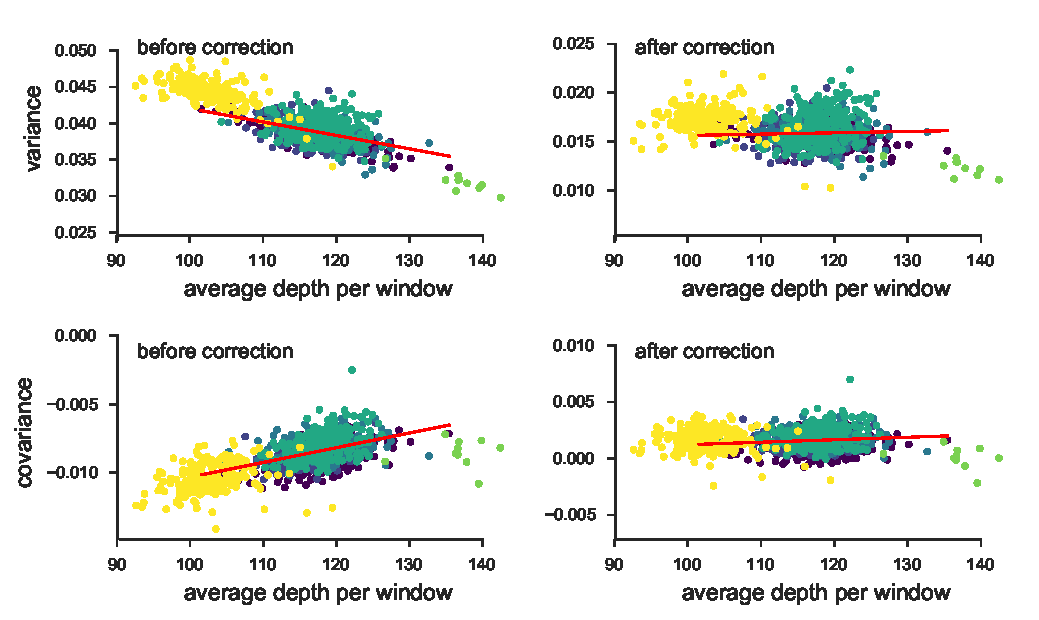
\includegraphics[]{figures/barghi-correction-plot.pdf}

  \caption{The variance and covariances from the \textcite{Barghi2019-qy}
    study, calculated in 100kb genomic windows plotted against average depth in
    a window before and after bias correction.  Each panel has a least-squares
    estimate between the variance and covariance, and the average depth.
    Overall, the bias correction corrects sampling bias in both the variance
    and covariance such that the relationship with depth is constant. Colors
    indicate the different chromosomes of \emph{D. simulans}; we have excluded
  the X chromosome (yellow points) and chromosome 4 points (green points to far
right) from the regression due to large differences in average coverage.}

  \label{suppfig:barghi-correction}
\end{figure}

\clearpage
\subsection{\textcite{Barghi2019-qy} Empirical Null and Windowed Covariance Distributions}

\begin{figure}[!ht]
  \centering
  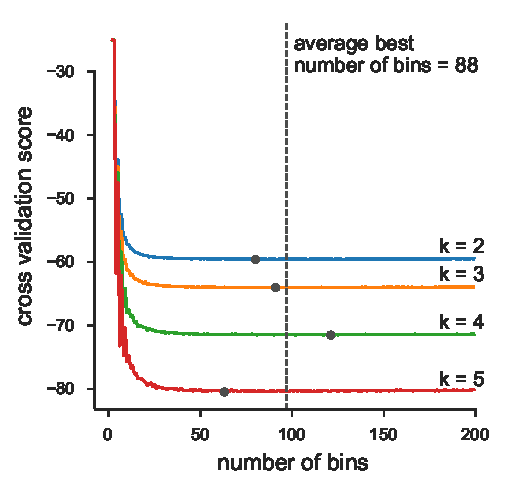
\includegraphics[]{figures/barghi-cross-validation-binsize.pdf}

  \caption{We chose number of bins used in the histograms of Figure
    \ref{fig:figure-3} via an analytic expression for the cross-validation
    risk, based on the equation 6.16 of (\cite{Wasserman2006-jl}, p. 129).
    Above, we plot the cross-validation risk for various numbers of bins, for
    each of the four off-diagonals of the temporal covariance matrix that we
    analyze. Overall, because the number of data points is large, oversmoothing
    is less of a problem, leading the cross-validation risk to be relatively
    flat across a large number of bins. Each gray point indicates the minimal
    risk for a particular off-diagonal, and the dashed line indicates the best
    average binwidth across off-diagonals.}
  \label{suppfig:barghi-cross-validation-binsize}
\end{figure}



\begin{figure}[!ht]
  \centering
  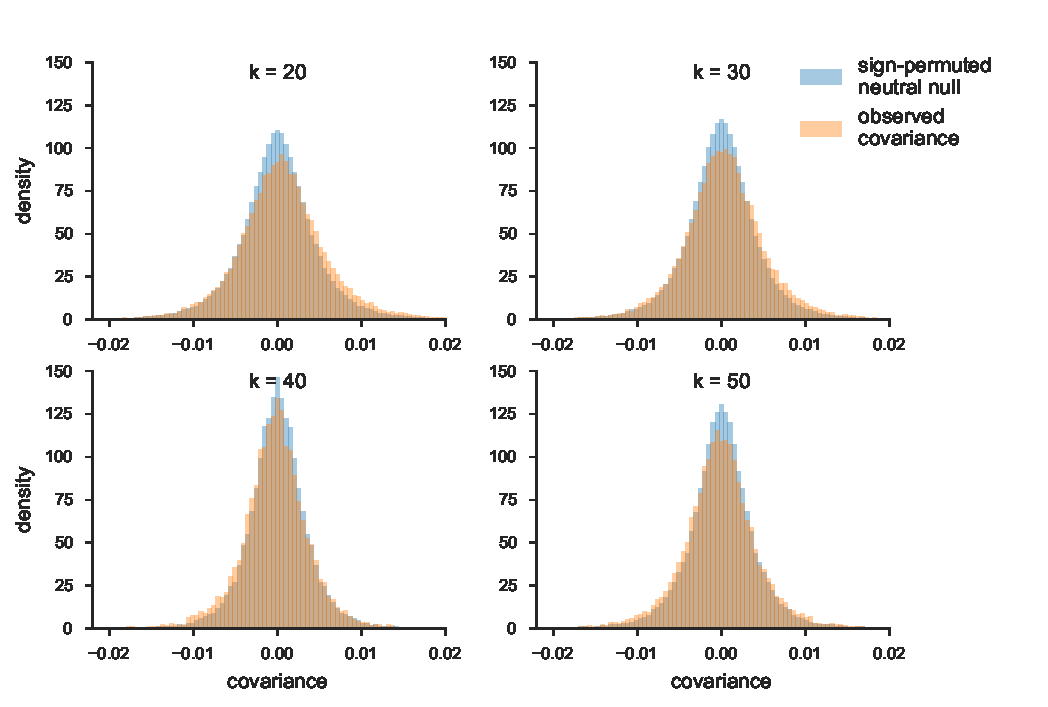
\includegraphics[]{figures/barghi-offset-panels.pdf}

  \caption{The distribution of temporal covariances calculated across 100kb
    genomic windows from \textcite{Barghi2019-qy}'s study (orange) and the
    block sign permuted empirical neutral null distribution of the windowed
    covariances (blue). Each panel shows these windowed covariances and the
    empirical null distribution for covariances $\cov(\Delta p_t, \Delta p_{t+k})$,
  $k$ is the number of generations between allele frequency changes.}
  \label{suppfig:barghi-empnull-tilecovs}
\end{figure}


\begin{figure}[!ht]
  \centering
  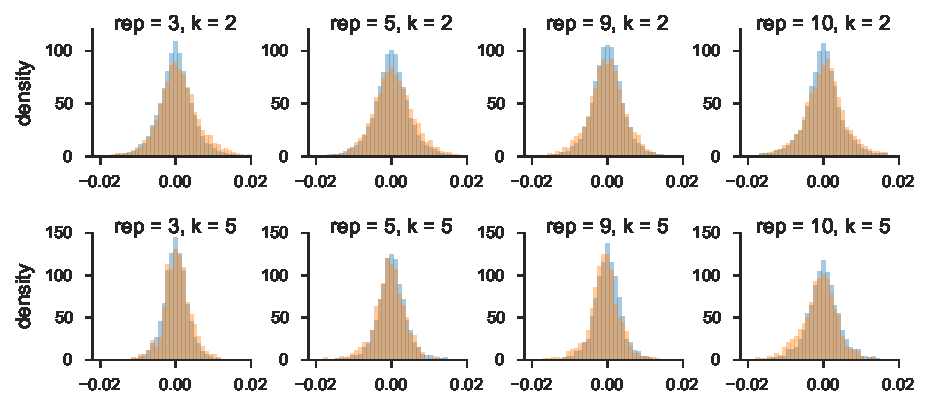
\includegraphics[]{figures/barghi-offset-replicate-panels.pdf}

  \caption{The distribution of windowed temporal covariances alongside the
    empirical neutral null for five randomly sampled replicates (columns), for
    $k=2$ (first row) and $k=5$ (second row). The main figure of the paper
    pools all replicate window and empirical neutral null covariances; we show
    here the windowed temporal covariances tend to shift from being positive (a
    heavier right tail) to become more negative (a heavier left tail) through
    time within particular replicates.}
  
  \label{suppfig:barghi-offset-replicate-panels}
\end{figure}


\begin{figure}[!ht]
  \centering
  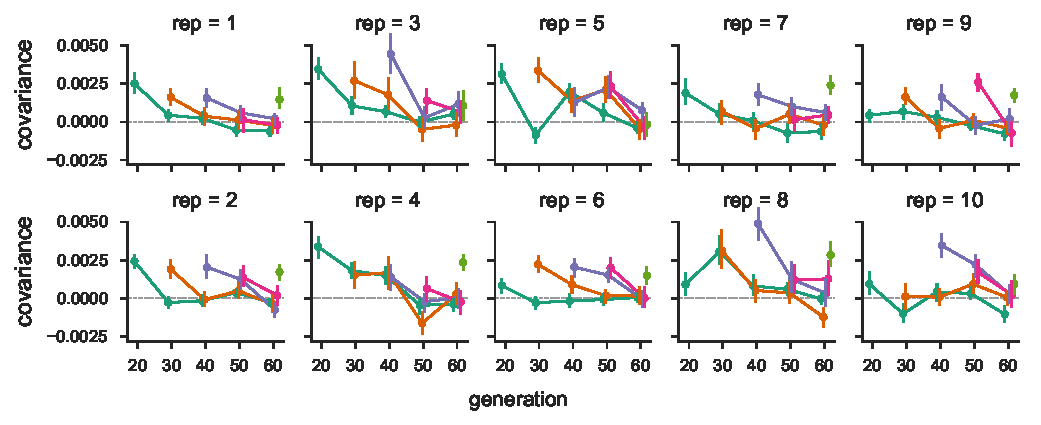
\includegraphics[width=\textwidth]{figures/barghi-cov-panels.pdf}

  \caption{The temporal covariances from the \textcite{Barghi2019-qy} study,
  for each replicate individually. As in Figure \ref{fig:figure-1}, each line
  follows the temporal covariances from some initial reference generation through
  time, which represent the rows of temporal covariance matrix.}

  \label{suppfig:barghi-cov-panels}
\end{figure}


\clearpage
\subsection{\textcite{Barghi2019-qy} Tail Probabilities for Windowed Covariances Distributions}

\begin{figure}[!ht]
  \centering
  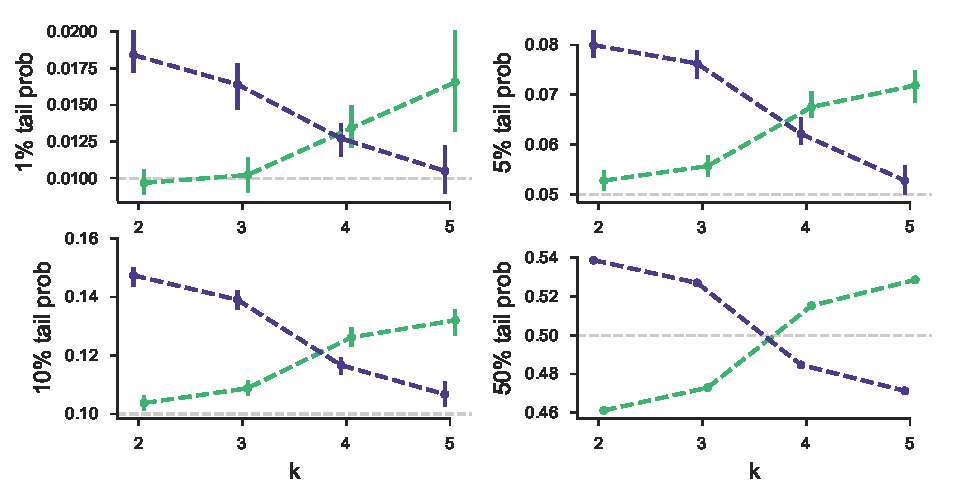
\includegraphics[]{figures/barghi-tailprobs-panels.pdf}

  \caption{\textcite{Barghi2019-qy} tail probabilities compared to
  sign-permuted empirical null distribution for various $\alpha$ levels.}

  \label{suppfig:barghi-tailprobs-panels}
\end{figure}

\begin{figure}[!ht]
  \centering

  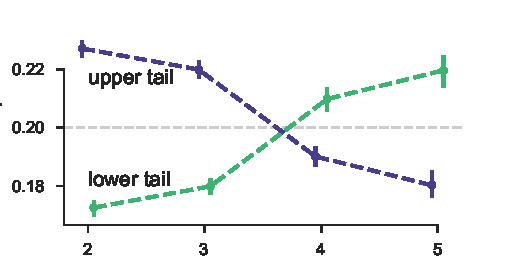
\includegraphics[]{figures/barghi-tailprobs-seqid-20.pdf}

  \caption{The 20\% lower and upper tail probabilities for the observed
  windowed covariances from the \textcite{Barghi2019-qy} study, based on
  sign-permuting at the chromosome level. This permutation empirical null
  is robust to long-range linkage disequilibrium acting over entire chromosomes.}
  
  \label{suppfig:barghi-tailprobs-seqid}
\end{figure}

\subsection{\textcite{Bergland2014-ij} Re-Analysis}
\label{supp:bergland-reanalysis}


We also applied our temporal covariance approach to \textcite{Bergland2014-ij},
which found evidence of genome-wide fluctuating selection between Spring and
Fall seasons across three years \emph{Drosophila melanogaster}. As described in
\textcite{Buffalo2019-io}, if fluctuating selection pressure among time-periods
are the dominant genome-wide pattern, we might expect positive covariances
between like seasons changes (e.g. Spring 2010 to Fall 2010 and Spring
2011 to Fall 2011), and negative covariances between dislike seasonal changes
(e.g. Fall 2009 to Spring 2010 and Fall 2010 to Spring 2011). However,
while we find temporal covariances that are non-zero, we find only weak support
for a seasonal fluctuating model driving these covariances. In Supplementary
Figure \ref{suppfig:bergland-covs-figure}, we show the temporal covariances
from varying reference generations, across seasonal transitions that are alike
(e.g.  the covariance between the allele frequency changes between Fall 2009
and Spring 2009, and frequency changes between Fall 2010 and Spring 2010), and
dislike (e.g. the covariance between the allele frequency change between Fall
2009 and Spring 2009, and the frequency changes between Spring 2010 and Fall
2009). The first row of temporal covariance matrix is consistent with
fluctuating selection operating for two timepoints, as the first covariance is
negative, and the second is positive, and later covariances are not
statistically differentiable from zero (which could occur if LD and additive
genetic variance decay). However, the all other temporal covariances do not fit
the pattern we would expect under genome-wide fluctuating selection.

\begin{figure}[!ht]
  \centering
  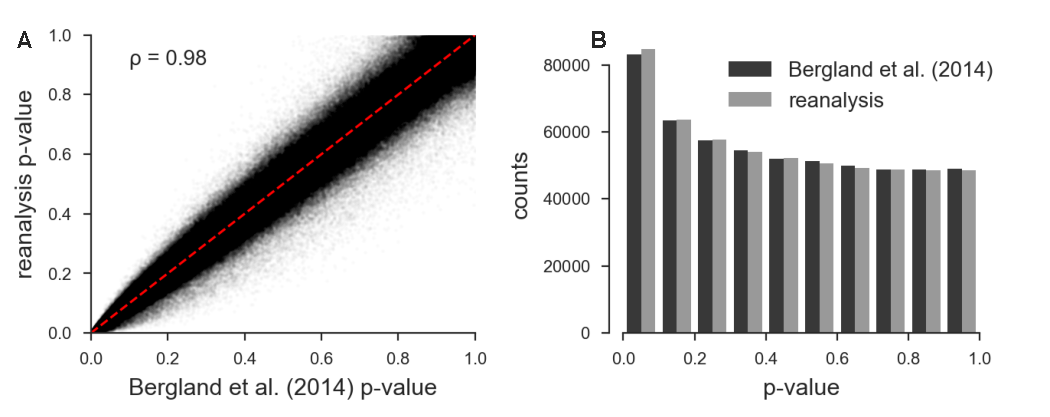
\includegraphics[width=\textwidth]{figures/bergland_pvalues.pdf}

  \caption{\textbf{A}: Scatterplot of the original unadjusted p-values from
    \textcite{Bergland2014-ij} and the p-values from our reanalysis of the same
    data using the same statistical methods; the minor discrepancy is likely
    due to software version differences. \textbf{B}: The histograms of the
    p-values of our reanalysis and the original \textcite{Bergland2014-ij}
    data; again the minor discrepancy is likely due to software differences.
    Overall, our implementation of Bergland et al.'s statistical methods
    produces results very close to the original analysis.}

  \label{suppfig:bergland-pvalue-comparison}
\end{figure}

We wanted to establish that our temporal-covariance matrix bias correction was
working correctly. We find that it corrects the relationship between depth and
both variance and covariance (Supplementary Figure
\ref{suppfig:bergland-correction}) as expected.

It is unclear how strong the fluctuations would have to be to generate a
genome-wide average signal of fluctuating selection from temporal covariances.
For example, many loci could still show a signal of fluctuating selection, but
the average signal could be overwhelmed by other signals of other selection. To
investigate whether there was an genome-wide excess of loci showing evidence of
fluctuating selection we reanalyzed the data of \parencite{Bergland2014-ij}
using the same seasonal fluctuating model as the original paper. This model is
a Binomial logit-linked GLM fit per-locus, where the Spring/Fall seasons are
encoded as a dummy variable, and are regressed on the frequency data. We use
the same binomial weighting procedure as \textcite{Bergland2014-ij}, where the
weights are determined by the effective number of chromosomes, $N_{eff} = (2
n_t d_t - 1) / (2 n_t + d_t)$ ($n_t$ and $d_t$ are the number of diploid
individuals and the read depth at timepoint $t$, respectively). We fit this
model on all loci marked as used in the VCF provided with the
\textcite{Bergland2014-ij} study (doi:10.5061/dryad.v883p). Overall, our
p-values for the Wald test for each locus closely match those of the original
paper (Pearson correlation coefficient 0.98, p-value < $2.2 \times 10^{-16}$;
see Supplementary Figure \ref{suppfig:bergland-pvalue-comparison} A), and the
histograms of the p-values are nearly identical (Supplementary Figure
\ref{suppfig:bergland-pvalue-comparison} B). \textcite{Bergland2014-ij} find
loci with a significant association with season after a Benjamini and Hochberg
FDR p-value adjustment \parencite{Benjamini1995-jy}, however, the null
hypothesis of the Wald test does not give us an idea of the expected number of
variants that may spuriously fit the pattern of seasonal fluctuating selection
as it does not account for genetic drift or other forms of hitchhiking.

% ======= We were concerned that this might be due to a flaw in our methods. To
% address this concern, we first ensured that our temporal-covariance matrix
% bias correction was working as expected. We find that it corrects the
% relationship between depth and both variance and covariance (Supplementary
% Figure \ref{suppfig:bergland-correction}) as expected. We then re-analyzed
% the data of \parencite{Bergland2014-ij} using the same seasonal fluctuating
% model as the original paper. This model is a Binomial logit-linked GLM fit
% per-locus, where the Spring/Fall seasons are encoded as a dummy variable, and
% are regressed on the frequency data. We use the same binomial weighting
% procedure as \textcite{Bergland2014-ij}, where the weights are determined by
% the effective number of chromosomes, $N_{eff} = (2 n_t d_t - 1) / (2 n_t +
% d_t)$ ($n_t$ and $d_t$ are the number of diploid individuals and the read
% depth at timepoint $t$, respectively). We fit this model on all loci marked
% as used in the VCF provided with the \textcite{Bergland2014-ij} study
% (doi:10.5061/dryad.v883p).  Overall, our p-values for the Wald test for each
% locus closely match those of the original paper (Pearson correlation
% coefficient 0.98, p-value < $2.2 \times 10^{-16}$; see Supplementary Figure
% \ref{suppfig:bergland-pvalue-comparison} A), and the histograms of the
% p-values are nearly identical (Supplementary Figure
% \ref{suppfig:bergland-pvalue-comparison} B).  >>>>>>>
% d95c3549a10dc0037f40a54cb8b41f9d412ed1ed

\begin{figure}[!ht]
  \centering
  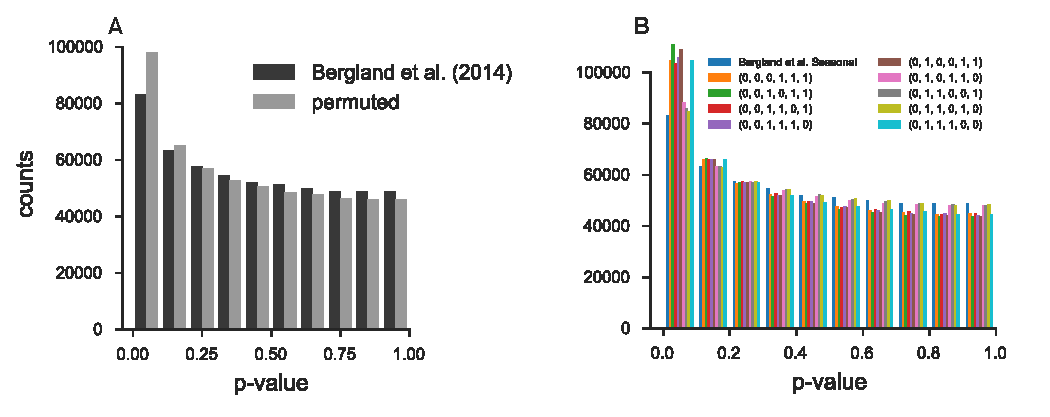
\includegraphics[width=\textwidth]{figures/bergland-combined-hists.pdf}

  \caption{\vb{\textbf{A}: Histogram of original \textcite{Bergland2014-ij}
    seasonal p-values and p-values creating by randomly permuting the seasons
    at each locus. \textbf{B}: Histogram of original \textcite{Bergland2014-ij}
    p-values alongside all unique permutations (ignoring symmetries that lead
    to identical p-values).}}

  \label{suppfig:bergland-pvalue-hist}
\end{figure}


\begin{figure}[!ht]
  \centering
  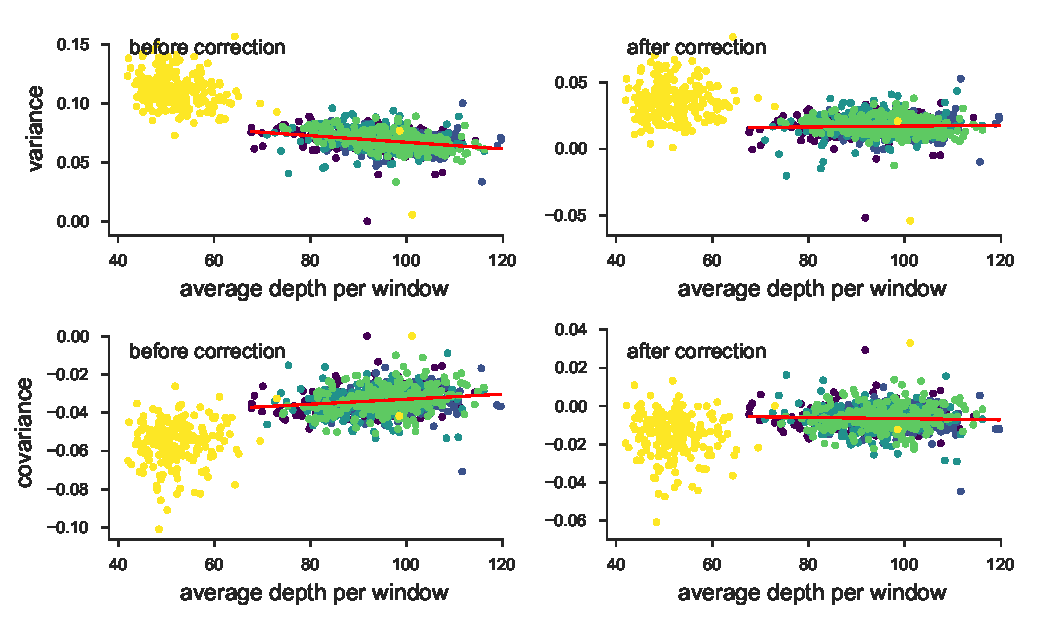
\includegraphics[width=\textwidth]{figures/bergland-correction-plot.pdf}

  \caption{The variance and covariances from the \textcite{Bergland2014-ij}
    study, calculated in 100kb genomic windows plotted against average depth in
    a window before and after bias correction. Each panel has a least-squares
    estimate between the variance and covariance, and the average depth.
    The bias correction procedure is correcting sampling bias in both the variance
    and covariance such that the relationship with depth is constant. Colors
    indicate the different chromosomes of \emph{D. melanogaster}; we have
    excluded the X chromosome (yellow points; chromosome 4 was not in the
    original study) from the regression due to large differences in average
    coverage.}

  \label{suppfig:bergland-correction}
\end{figure}



To investigate whether there is a genome-wide evidence of an enrichment of
fluctuating selection we created an empirical null distribution by randomly
permuting the season labels and re-running the per-locus seasonal GLM model, as
proposed by \textcite{Machado2018-cs}. We find, regardless of whether we
permute at the locus-level or the permutation replicate-level, that the
observed seasonal p-value distribution \textcite{Bergland2014-ij} is not
enriched for significant p-values beyond what we would expect from the
permutation null. In fact, there appears there is more enrichment for low
p-values when seasonal labels are randomly permuted (Supplementary Figure
\ref{suppfig:bergland-pvalue-hist}, suggesting by random chance we might expect
more variants with a seasonal fluctuating pattern than found in the original
\textcite{Bergland2014-ij} study. While surprising, this could be explained by
the presence of temporal structure across the samples not consistent with
seasonal fluctuating selection. Some fraction of the permutations happen to fit
this structure well, leading to an enrichment of small p-values. This
non-seasonal temporal structure is also evident in our temporal covariances
(Supplementary Figure \ref{suppfig:bergland-covs-figure}), where we see strong
evidence of selection (non-zero temporal covariances), yet the pattern does not
follow that of seasonal fluctuating selection.  

%\gc{ADD MORE HERE} TODO

\begin{figure}[!ht]
  \centering
  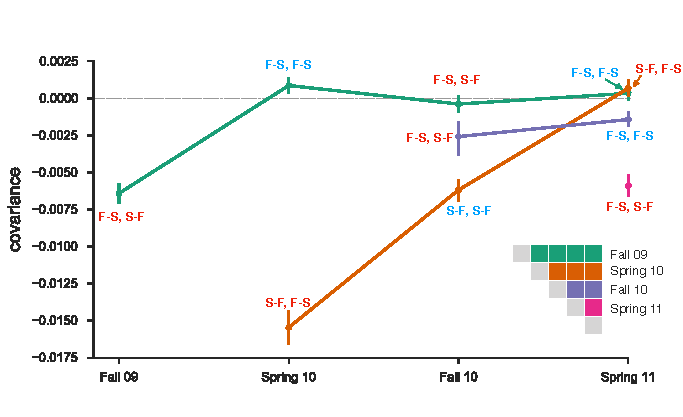
\includegraphics[]{figures/bergland-covs-figure.pdf}

  \caption{Temporal covariances from the \textcite{Bergland2014-ij} study, from
    varying reference generations (e.g. rows along the temporal covariance
    matrix). Each covariance is labeled indicating whether the covariance is
    between two like seasonal transitions (e.g. the covariance between allele
    frequency changes from fall to spring in one year, and fall to spring in
    another or two dislike seasons (e.g. the covariance between fall to spring
    in one year, and spring to fall in another year). Covariances between like
    transitions are expected to be positive when there is a genome-wide effect
    of fluctuating selection (and these labels are colored blue), while
    covariances between dislike transitions are expected to be negative (and
    these labels are colored red). 95\% confidence intervals were constructed
    by a block-bootstrapping procedure where the blocks are megabase tiles.}

  \label{suppfig:bergland-covs-figure}
\end{figure}



%\gc{Note that this analysis does not rule out the idea that prior
 % analyses detected {\emph
  %  some} loci showing a pattern of fluctuating selection. Indeed
  %\textcite{Bergland2014-ij} provided a number of analyses that
  %suggested that their loci might be enriched for {\bf XXX}. However,
  %this reanalysis suggests that we currently lack genome-wide evidence
%of many loci experiencing fluctuating selection in {\it in Drosophila
 % melanogaster}. }

\end{document}
